% Writeup for MDS
% David Lawrence Miller
% d.l.miller@bath.ac.uk
 
% Started : 22 August 2008
 
\documentclass[a4paper,10pt]{amsart}
 
% Load some packages
\usepackage{times, amsmath, amssymb, amsfonts, url, natbib, bm, rotating}
 
\usepackage{multirow}
\usepackage{graphicx}

% top matter
\title{Multidimensional scaling as a tool for smoothing over complex regions}
\author{David Lawrence Miller}
\email{d.l.miller@bath.ac.uk}
\address{Mathematical Sciences, University of Bath, Bath, United Kingdom}
 
% Shortcuts
% Probability
\newcommand{\prob}[1]{\mathbb{P}\left[ #1 \right]}
	% Hovitz-Thompson
\newcommand{\HT}{\hat{\tau}_{HT}}
% Schwarz-Christoffel
\newcommand{\sch}{Schwarz-Christoffel }
% fprime
\newcommand{\fprime}{f^\prime(z)}
% figure reference command
\newcommand{\fig}[1]{\emph{fig.} (\ref{#1})}
% Figure reference command
\newcommand{\Fig}[1]{\emph{Fig.} (\ref{#1})}
% equation reference command
\newcommand{\eqn}[1]{\emph{eqn.} (\ref{#1})}
% phi inverse
\newcommand{\phiinv}{\phi^{-1}}
% use other phi
\renewcommand{\phi}{\varphi}
%transpose
\newcommand{\tr}[1]{#1^{\text{T}}}
% diagonal
\newcommand{\diag}{\text{diag}}
% call \times \cross
\newcommand{\cross}{\times}


\begin{document}
 
% The abstract
\begin{abstract}
Here.
\end{abstract}
 
 
% New theorem for theorems
\newtheorem{thm}{Theorem}[section]
 
%New theorem for definitions
\newtheorem{defn}{Definition}[section]
 
\maketitle

%\markright{TECH. DETAILS OF SCHWARZ-CHRISTOFFEL MAPPING}

\section{Introduction}

Multidimensional scaling (MDS) or as it is often referred to principle coordinates (PCO) is a method commonly used in multivariate analysis to find a new configuration of points based on the distances between the points (\cite{chatfieldcollins}, p. 187.) In this new configuration, the Euclidean inter-point distances are approximately the same as their distances in the original data. Most often, MDS is used as a dimension reduction technique, finding a set of points in a lower dimension than the data, while still retaining information about the distances between the points. It is closely related to other methods such as PCA (\cite{chatfieldcollins}, p. 200) and canonical correspondance analysis (\cite{terbraak}.)

This method provides an obvious framework for the problem of smoothing over a region with a complex boundary. We can use the within-area distances to configure the points in such a way that smoothing does not suffer from leakage.

\section{Multidimensional Scaling}

The basic concept behind MDS is to take the data, represent them as a set of inter-point distances and then find a new coordinate system based on those inter-point distances. We do this by simply performing an eigen-decomposition on the matrix of distances between points.

\subsection{Finding the new point configuration}

We first define $d_{ij}$ as the distance between the points $i$ and $j$. These form a matrix, $D$, with $ij^{\text{th}}$ element $d_{ij}$. How we find $d_{ij}$ is discussed in the next section, for the moment we assume that we know $d_{ij}$.

\cite{diaconis08} gives a clear definition of the algorithm (due to \cite{schoenberg35}) for finding the new locations of points given we know the $d_{ij}$s. 

Taking the unknown new locations and putting them in an $n \times p$ matrix, $X$. Let $S=X\tr{X}$, and performing an eigen-decomposition we can see that $S=U\Lambda\tr{U}$. We may then represent $S$ in some arbitrary number of dimensions, $k$, by picking the $k$ largest eigenvectors of $S$. In this case, we are interested in

\begin{equation}
\tilde{X}=\tilde{U}\tilde{\Lambda}^{1/2}.
\end{equation}

where a tilde indicates the $n \times k$ versions of $X$, $\Lambda$ and $U$.

We can relate $D$ to $S$ by first defining

\begin{equation}
H = I-\frac{1}{n}\mathbf{1}\tr{\mathbf{1}}.
\end{equation}

By pre- and post-multiplying any matrix by $H$ we double centre it (row and column means are 0.) We then obtain\footnote{See \cite{diaconis08} for a simple proof.}:

\begin{equation}
S = -\frac{1}{2}HDH.
\end{equation}

So, in order to obtain a the new configuration of points using MDS (given that we have some set of inter-point distances) we merely need to double centre the matrix of distances and perform an eigen-decomposition.

Multidimensional scaling may be performed in \textsf{R} using the \texttt{cmdscale} function. 

\subsection{Inserting new points into the configuration}

Clearly, we may be in a position where the new coordinate system has been found by MDS but more data has been collected afterward. In this case we would like to insert those new points into the configuration given by MDS. This is relatively easy given we have the correct quantities for calculation.

We may find the new configuration, $\tilde{X}_{\text{new}}$, of some new data $X_{\text{new}}$ using:

\begin{equation}
\tilde{X}_{\text{new}} = \frac{1}{2} \Lambda^{-1} \tr{X} \mathbf{d},
\end{equation}

here $\Lambda$ and $\tr{X}$ are as above, $\mathbf{d}$ is defined as the vector of distances between each point in $X_{\text{new}}$ and the points in the original $X$ (\cite{gower1968}.) This formula is commonly referred to as ``Gower's interpolation.''

Although the calculation is simple, it hides two important pitfalls. First, if the eigenvectors in $\Lambda$ are not the true eigenvectors then we may insert points incorrectly. For example, if the sample is taken from only half of the space, since we don't have full information about the domain or, more pathologically, there were a trend in the sample locations. This would lead to the incorrect eigenvectors being obtained.

Second, if we insert new points that are equidistant from points already in the MDS, then the new point will be placed between the previously inserted points in the plane. This is fine when that is its true location, however it is possible that the point was supposed to not lie in the plane but rather in an extra dimension and its distance was truncated. An example of this is illustrated in \fig{bojinsert}. A more complete explanation and characterization of this problem is given in \cite{Boj2009}.

The effects of the above problems can be seen in \fig{wt2zoom} for the domain in \fig{wt2dia}. This shows that the $\Lambda$ found does not explain enough of the variation in that part of the domain, thus squashing the points together.

% zoom of the insertion error in wt2.
\begin{figure}
\centering
% trim order l b r t
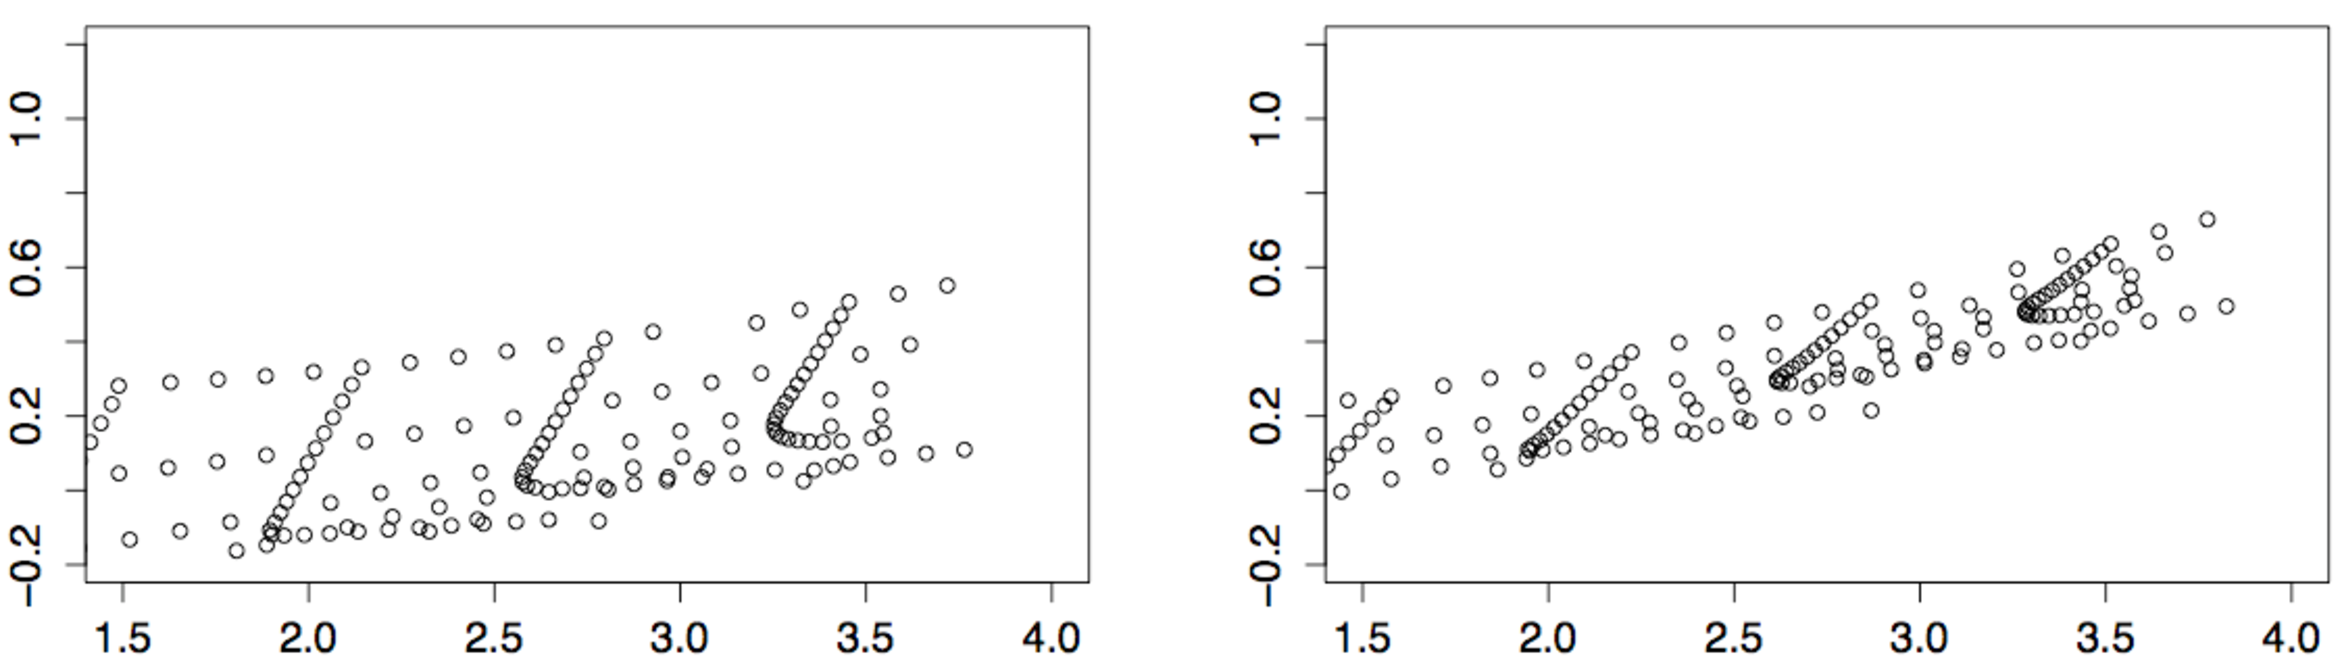
\includegraphics[width=5in]{figs/wt2-zoom.pdf}\\
\caption{Zoom of the mapping of a grid on the domain shown in \fig{wt2dia}. The left panel shows when the whole domain has been mapped as one and then the grid found by insertion, the second uses only the sample to construct the MDS and then again the location of the grid points is found by insertion.}
\label{wt2zoom}
\end{figure}


For the above reasons, Gower's interpolation is not used on the sample alone. Rather, a representative set of points are used when constructing $\Lambda$. This approach removes the sensitivity of the fit to the location of the points in the sample.

% diagram from Boj et al. 2009
\begin{figure}
\centering
% trim order l b r t
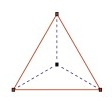
\includegraphics{figs/boj0.jpg} 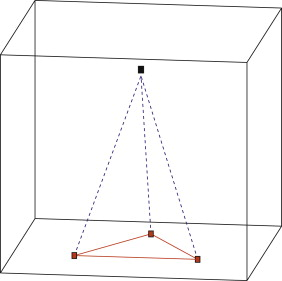
\includegraphics[width=1in]{figs/boj1.jpg} \\
\caption{Given the three points that make up the equilateral triangle in the left panel, if a new point is introduced then it will be placed in the centre of those points, even if it's distance from all old points is much greater (see right panel.) This is due to the projection onto the sample eigenvectors. Taken from \cite{Boj2009}.}
\label{bojinsert}
\end{figure}




\section{Finding the within-area distances}

The within-area distances to be fed to MDS are found using a novel algorithm. This works by tracing the inside sides of the polygon and then modifying the path by deleting and replacing portions of the path. Given that there is no direct path within the domain ($\Gamma$, say) between two points ($p_1$ and $p_2$, say), the algorithm proceeds as follows:

\begin{itemize}
\item Create initial path by drawing a line between $p_1$ and $p_2$ (\fig{wdia}, ($i$)) and where they meet the boundary of $\Gamma$ and start the path as the lines from $p_1$, $p_2$ to their first intersection with the boundary of $\Gamma$. Then find the distance between these two intersection points in both directions, along the boundary (\fig{wdia}, ($ii$).) Choose the shorter of these add the paths between $p_1$, $p_2$ and the boundary and this is the starting path(\fig{wdia}, ($iii$).) 
\item Given a triple of vertices, $v_1$, $v_2$, $v_3$ if the line between $v_1$ and $v_3$ is shorter than the path ($v_1$, $v_2$, $v_3$) and the line between $v_1$ and $v_3$ lies inside $\Gamma$ then delete $v_2$ (\fig{wdia}, ($iv$) and ($vi$).) This iterates over the entire path once, deleting all superfluous vertices. 
\item Given a triple of vertices, $v_1$, $v_2$, $v_3$ if the path $v_1$, some subset of the vertices of $\Gamma$, $v_3$ is shorter than the path ($v_1$, $v_2$, $v_3$) then replace $v_2$ with those elements of $\Gamma$ (\fig{wdia}, ($v$)). 
\item We then iterate between steps 2 and 3 until there has been no change from one run to the next (ie. convergence) or there have been too many iterations (\fig{wdia}, ($vi$).)
\end{itemize}

% diagram for finding the shortest path in W
\begin{figure}
\centering
% trim order l b r t
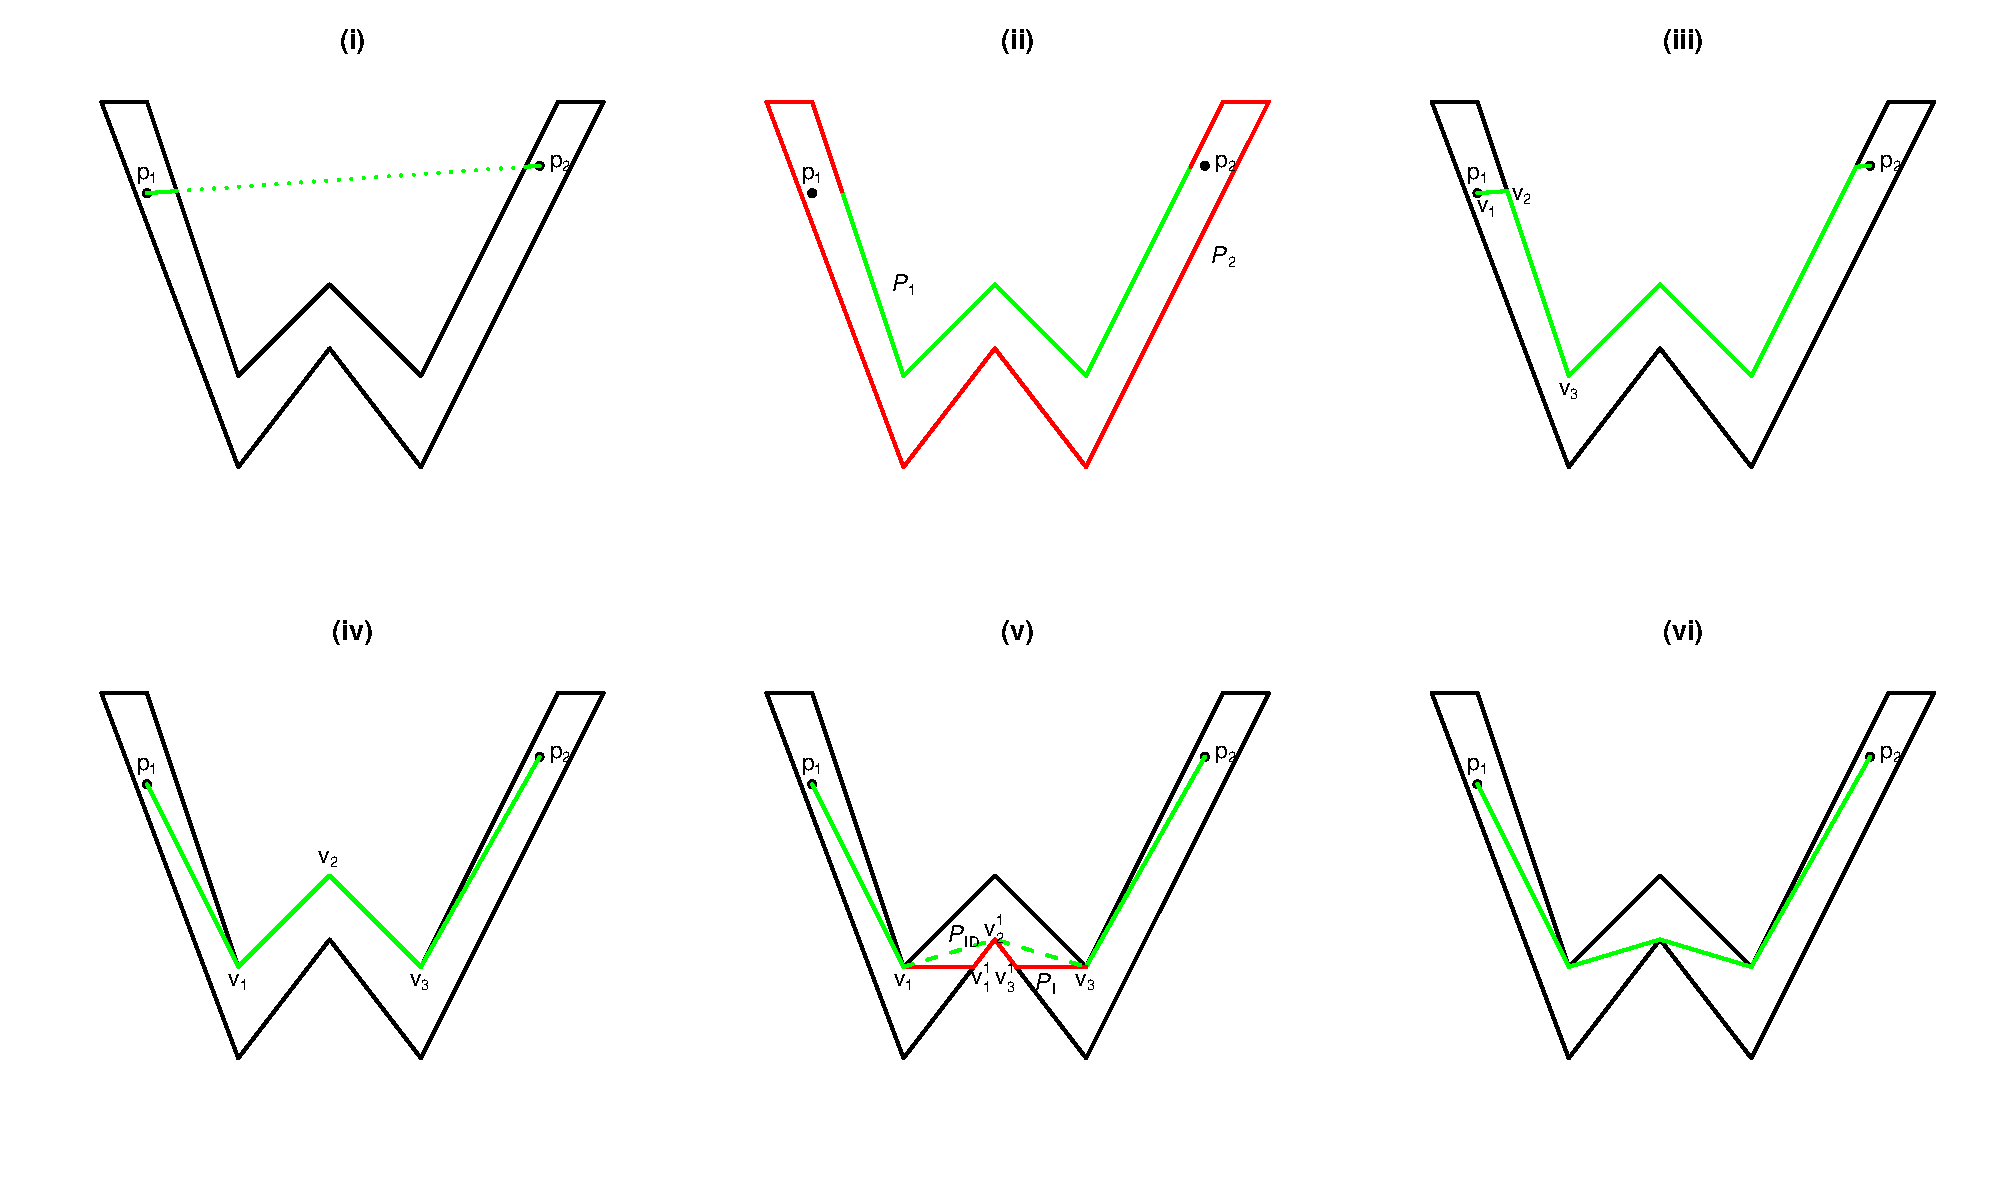
\includegraphics[trim=0in 0.5in 0in 0.25in, width=4in]{figs/wdia.pdf} \\
\caption{($i$) to ($vi$) show the path as the algorithm progresses from initial state to final, shortest path. }
\label{wdia}
% generate /phd-smoothing/mds-writeup/figs/distanceexplanation.R
\end{figure}



[[ euclidean distance analysis ]]


\section{Multidimensional scaling for complex domains}

Tying together the two previous sections, we may now look at how, using MDS and our new algorithm, we can reconfigure the points in our domain.

\Fig{ramsay-mds} shows MDS being performed on the Ramsay horseshoe (\cite{ramsay}.) From this it is clear to see that performing MDS separates the two arms of the horseshoe.

% Ramsay MDSed 
\begin{figure}
\centering
% trim order l b r t
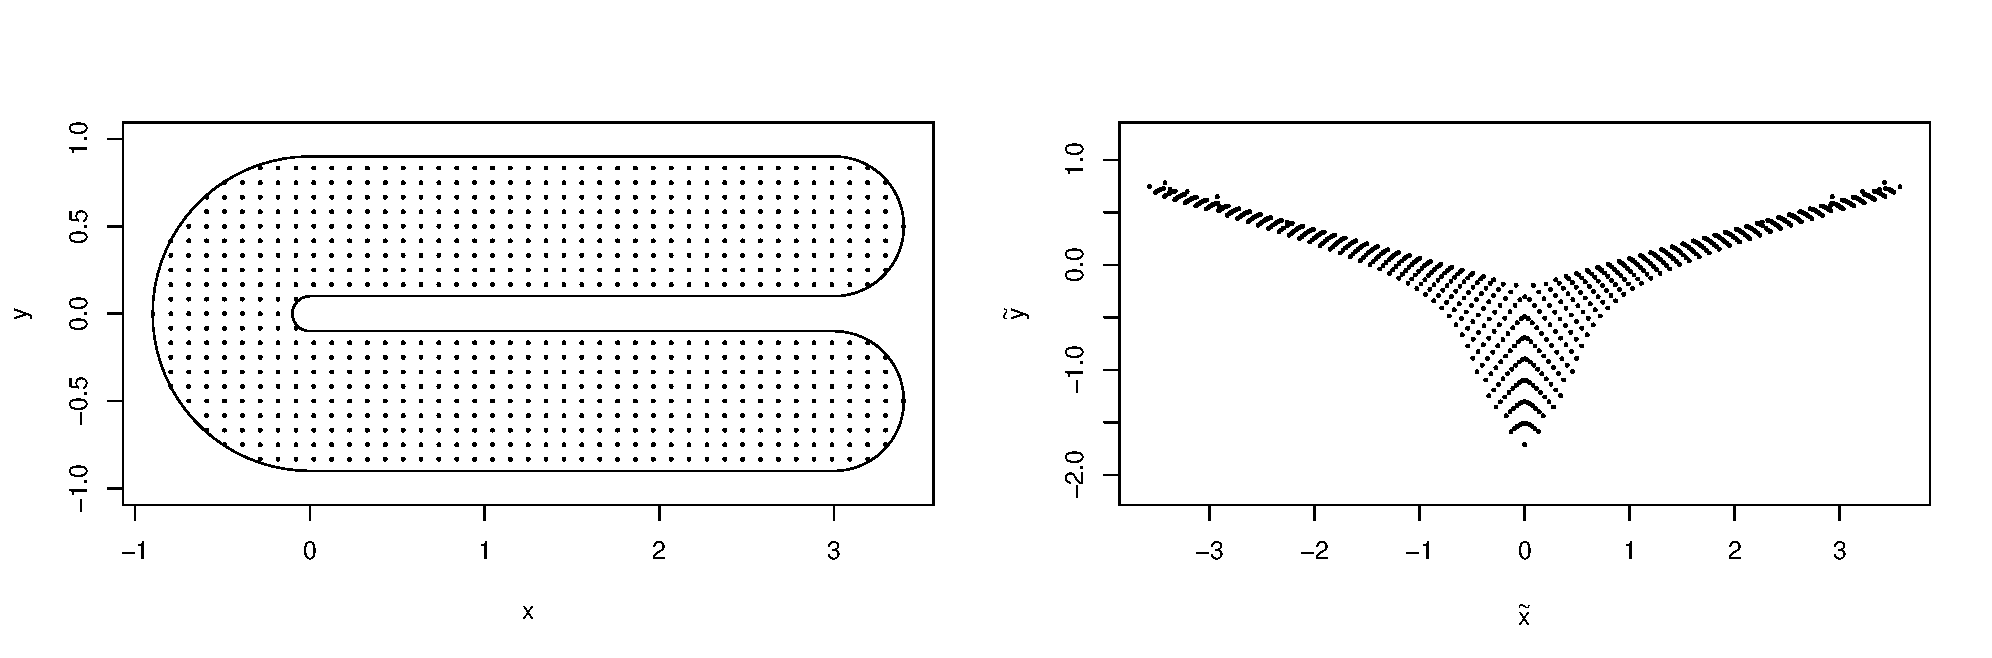
\includegraphics[trim=0in 0.5in 0in 0.25in, width=5.5in]{figs/ramsay-mds.pdf} \\
\caption{Left panel shows the horseshoe with 734 points. Right panel shows their configuration under MDS using the algorithm detailed above.}
\label{ramsay-mds}
% generate /phd-smoothing/mds-writeup/figs/ramsay-mds.R
\end{figure}

An advantage of the MDS approach is that in our eigen-decomposition we may pick an arbitrary number of eigenvectors to retain and push the original set of points into higher dimensions. Using three eigenvectors we get the configuration in \fig{ramsay-mds-3d}.

The two eigenvalues returned from running \texttt{cmdscale} in \textsf{R} when we ask for a 2-dimensional are 2615.5597 and 229.0039. Adding another dimension gives eigenvalues of 2615.5597, 229.0039, 46.8754. Clearly significantly less variation is being explained in the third dimension, however this may well not be of primary concern if it prevents leakage.


\Fig{wt2dia} shows another domain which is more complicated than the horseshoe. The region has peninsulae which will cause similar problems to those found in the horseshoe. 




% Ramsay MDSed 
\begin{figure}
\centering
% trim order l b r t
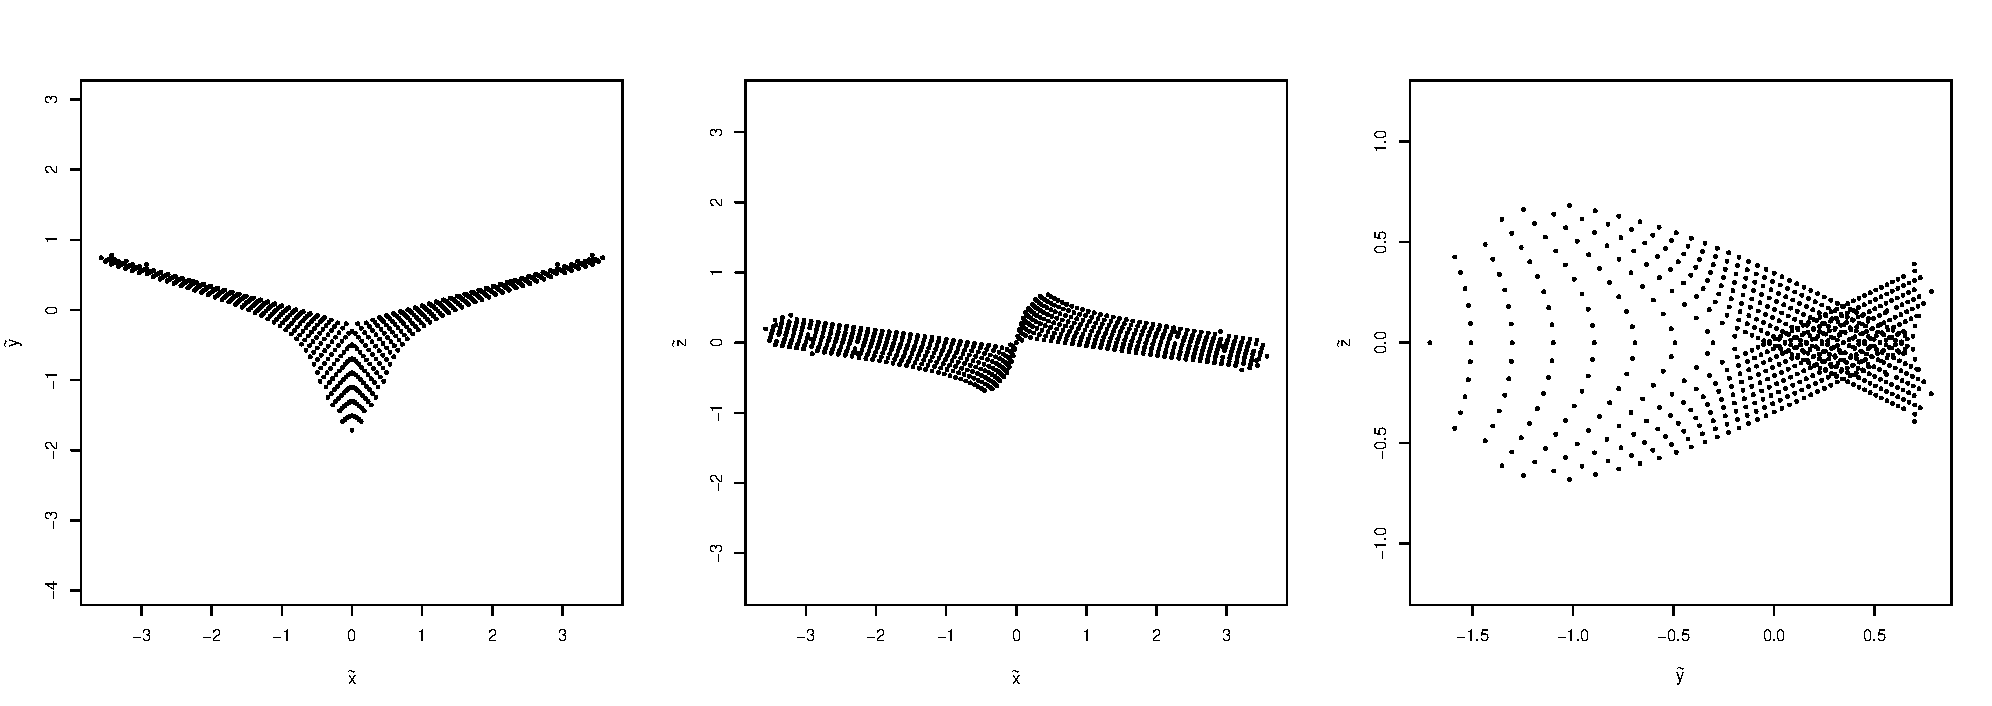
\includegraphics[trim=0in 0.5in 0in 0.25in, width=5.5in]{figs/ramsay-mds-3d.pdf} \\
\caption{Two-dimensional projections of the 3D mapping of the horseshoe.}
\label{ramsay-mds-3d}
% generate /phd-smoothing/mds-writeup/figs/ramsay-mds.R
\end{figure}

% plot of points in wt2.
\begin{figure}
\centering
% trim order l b r t
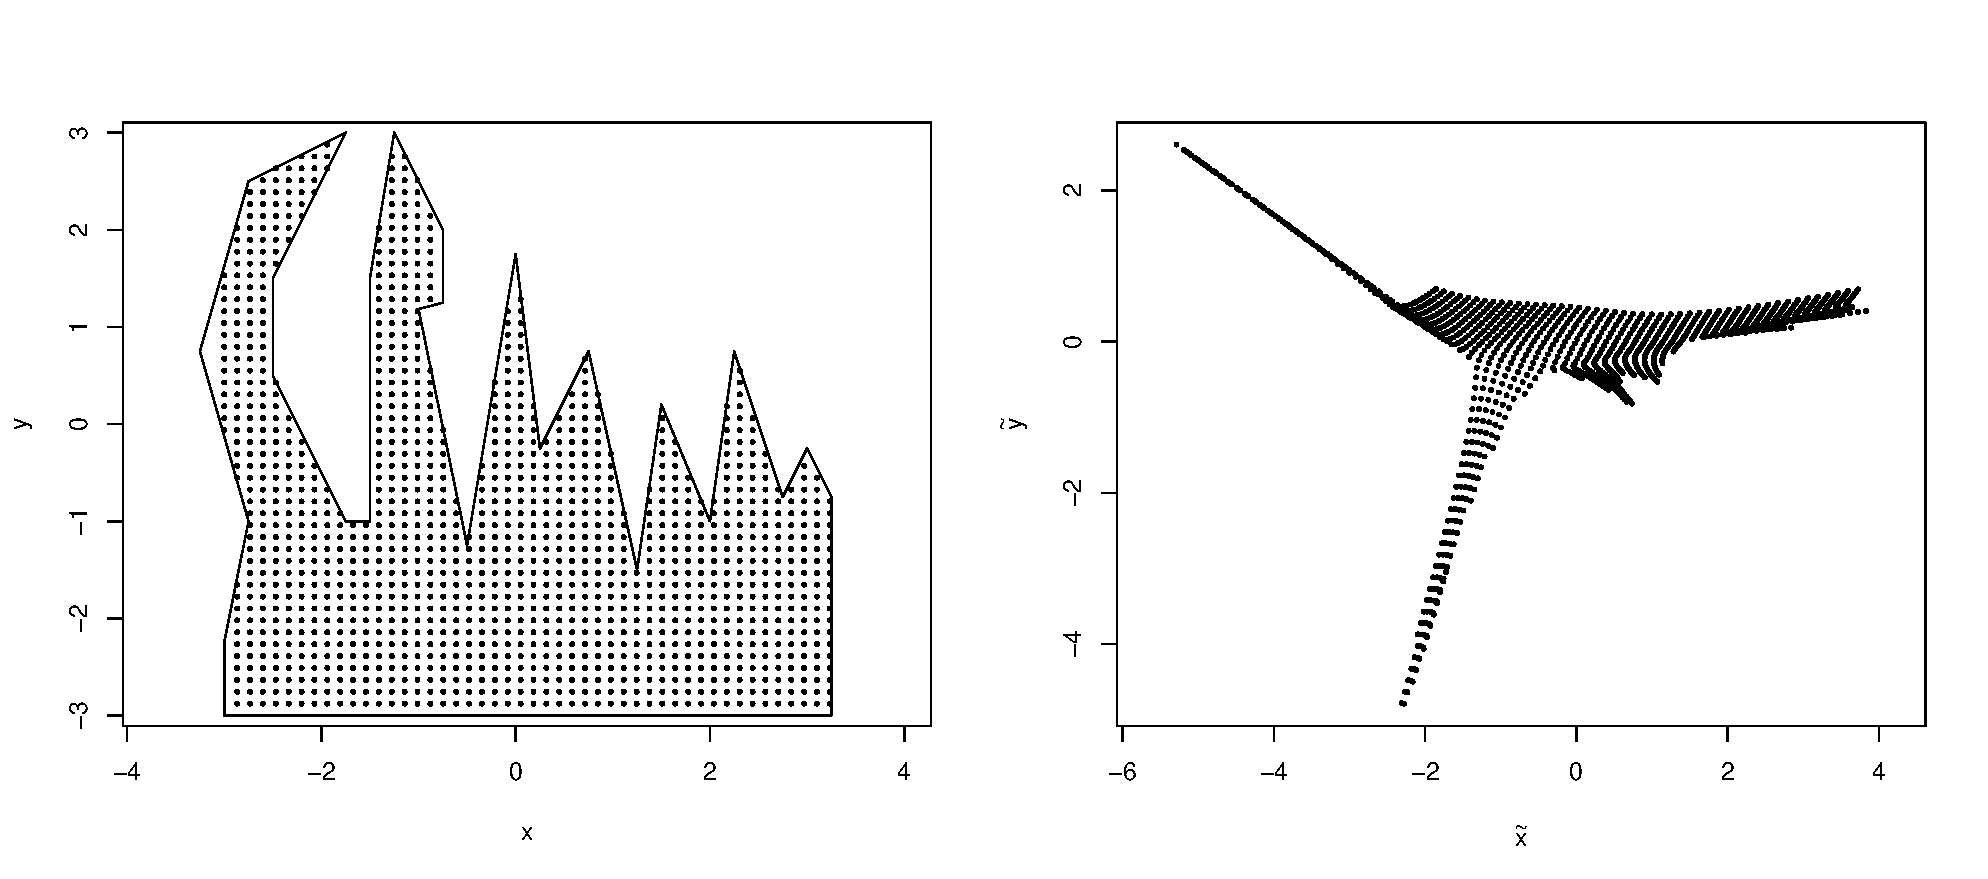
\includegraphics[width=6in]{figs/wt2-mds.pdf}\\
\caption{A domain with many peninsulae (left), and its MDS projection in two dimensions (right) for 1253 points in the domain.}
\label{wt2dia}
\end{figure}








\section{Simulation experiment}


VVVVV one run only

Ramsay
mds MSE= 0.002239077 
tprs MSE= 0.0651262 
soap MSE= 0.001455530 


wt2
mds=0.1291663
tprs=0.0760142
soap=0.02217734


3d sims

 summary(res.mse.mds)
   Min. 1st Qu.  Median    Mean 3rd Qu.    Max. 
0.04568 0.06914 0.08467 0.09712 0.10440 1.16000 
 summary(res.mse.tprs)
   Min. 1st Qu.  Median    Mean 3rd Qu.    Max. 
0.04369 0.06505 0.07444 0.07898 0.08667 0.28870 
 summary(res.mse.soap)
    Min.  1st Qu.   Median     Mean  3rd Qu.     Max. 
 0.01757  0.02123  0.02336  0.04722  0.02759 10.12000 





do plots of vis.gam() with too.far set low and overlay of points

boxplots



\section{Conclusions}


\bibliographystyle{plainnat}
\bibliography{mds-refs}

\end{document}
